% Created 2016-11-07 Mon 13:50
% Intended LaTeX compiler: pdflatex
\documentclass[12pt]{report}
\usepackage[utf8]{inputenc}
\usepackage[T1]{fontenc}
\usepackage{graphicx}
\usepackage{grffile}
\usepackage{longtable}
\usepackage{wrapfig}
\usepackage{rotating}
\usepackage[normalem]{ulem}
\usepackage{amsmath}
\usepackage{textcomp}
\usepackage{amssymb}
\usepackage{capt-of}
\usepackage{hyperref}
\usepackage{geometry}
\usepackage[activate={true,nocompatibility},final,tracking=true,kerning=true,spacing=nonfrench,factor=1100,stretch=10,shrink=10]{microtype}
\usepackage{minted}
\usepackage{aums}
\usepackage{natbib}
\usepackage[dvipsnames]{xcolor}
\usepackage{algorithm}
\usepackage{algorithmic}
\usepackage{caption}
\usepackage{subcaption}
\usepackage{threeparttable}
\renewcommand\maketitle{}

\copyrightyear{2016}

\keywords{data cleansing, range query, \(k\)NN query, particle filter,
Kalman filter}

\adviser{Dr. Wei-Shinn Ku}

\professor{Thaddeus Roppel, Chair, Associate Professor of Electrical
and Computer Engineering}

\professor{Prathima Agrawal, Ginn Distinguished Professor of
Electrical and Computer Engineering}

\professor{John Hung, Professor of Electrical and Computer
Engineering}
\author{Zhitao Gong}
\date{\today}
\title{RFID data cleansing with Bayesian Filters}
\hypersetup{
      pdfauthor={Zhitao Gong},
      pdftitle={RFID data cleansing with Bayesian Filters},
      pdfkeywords={},
      pdfsubject={},
      pdfcreator={Emacs 24.5.1 (Org mode 9.0)},
      pdflang={English},
      bookmarks=true,
      unicode=true,
      pdftoolbar=true,
      pdfmenubar=true,
      pdffitwindow=false,
      pdfstartview={FitH},
      pdfnewwindow=true,
      colorlinks=true,
      linkcolor=Maroon,
      citecolor=ForestGreen,
      filecolor=Mulberry,
      urlcolor=MidnightBlue}
\begin{document}

\maketitle
\TitlePage

\begin{romanpages}


\begin{abstract}
People spend a significant amount of time in indoor spaces (e.g.,
office buildings, subway systems, etc.) in their daily lives.
Therefore, it is important to develop efficient indoor spatial query
algorithms for supporting various location-based applications.
However, indoor spaces differ from outdoor spaces because users have
to follow the indoor floor plan for their movements.  In addition,
positioning in indoor environments is mainly based on sensing devices
(e.g., RFID readers) rather than GPS devices.  Consequently, we cannot
apply existing spatial query evaluation techniques devised for outdoor
environments for this new challenge.  Because Bayesian filtering
techniques can be employed to estimate the state of a system that
changes over time using a sequence of noisy measurements made on the
system, in this research, we propose the Bayesian filtering-based
location inference methods as the basis for evaluating indoor spatial
queries with noisy RFID raw data.  Furthermore, two novel models,
indoor walking graph model and anchor point indexing model, are
created for tracking object locations in indoor environments.  Based
on the inference method and tracking models, we develop innovative
indoor range and \(k\) nearest neighbor (\(k\)NN) query algorithms.
We validate our solution through extensive simulations with real-world
parameters.  Our experimental results show that the proposed
algorithms can evaluate indoor spatial queries effectively and
efficiently.
\end{abstract}

\begin{acknowledgments}
I would like to thank Ms. Jiao Yu for her insightful discussion and
contribution.  We both work on this work.  Ms. Yu worked on the
particle filter and snapshot queries, while I focus on Kalman filter
and continuous queries.

In addition, I would also like to thank Dr. Ku for his invaluable
guidance during my research.  I learned how to think like a researcher
and how to narrow down areas of focus during our weekly discussion.  I
also greatly appreciate his patience for my really slow research
progress.
\end{acknowledgments}

\tableofcontents
\listoffigures
\listoftables
\end{romanpages}

\part{Introduction}
\label{sec:introduction}
Today most people spend a significant portion of their time in
indoor spaces such as subway systems, office buildings, shopping
malls, convention centers, and etc.  In addition, indoor spaces are
increasingly larger and more complex.  For instance, the New York
City Subway has 469 stations and 233 miles (375 km) of routes
\cite{wikipedia2016-new}.  In 2014, the subway system delivered over
1.75 billion rides, averaging approximately 5.6 million rides on
weekdays \cite{authority2014-subway}.  Therefore, users will have more
and more demand for launching spatial queries for finding friends or
Points Of Interest (POI) in indoor places.  Moreover, users are
usually moving around when issuing queries.  Thus we need to
properly support indoor spatial queries \emph{continuously}, e.g.,
reporting nearby friends in a mall when a user is shopping.
However, existing spatial query evaluation techniques for outdoor
environments (based on either Euclidean distance or network
distance)
\cite{roussopoulos1995-nearest,hjaltason1999-distance,papadias2003-query,samet2008-scalable,lee2012-road}
cannot be applied in indoor spaces because these techniques assume
that user locations can be acquired from GPS signals, which are not
available in indoor spaces.  Furthermore, indoor spaces are usually
modeled differently from outdoor spaces.  In indoor environment,
user movements are constrained by topology such as doors, walls, and
hallways.

Radio Frequency Identification (RFID) technologies have become
increasingly popular over the last decade with applications in areas
such as supply chain management \cite{santos2008-rfid}, health care,
and transportation.  In indoor environments, RFID is mainly employed
to support track and trace applications.  Generally, RFID readers
are deployed in critical locations where objects carry RFID tags.
When a tag enters the detection range of a reader, the reader
recognizes the presence of the tag and generates a record in the
backend database.  However, the raw data collected by RFID readers
is inherently unreliable \cite{jeffery2006-adaptive}, with false
negatives as a result of RF interference, limited detection range,
tag orientation, and other environmental phenomena
\cite{welbourne2009-building}.  In addition, readers cannot cover all
areas of interest because of their high cost or privacy concerns.
Therefore, with RFID raw data, we cannot provide reliable support
for commonly used spatial query types, e.g., range and \(k\)NN in
indoor environments.  Several other types of wireless communication
technologies such as WiFi and Bluetooth have been employed for
indoor positioning \cite{anastasi2003-experimenting,bell2010-wifi}.
However, each aforementioned technology has considerable positioning
uncertainty.  Furthermore, WiFi and Bluetooth are mainly utilized
for locating individual users rather than supporting a centralized
indoor location tracking system.  It is too expensive to attach WiFi
or Bluetooth transmitters (\$5 per device) to monitored objects.
Therefore, we focus on RFID in this research.

In this paper, we consider the setting of an indoor environment
where a number of RFID readers are deployed in hallways.  Each user
is attached with an RFID tag, which can be identified by a reader
when the user enters the detection range of the reader.  Given the
history of RFID raw readings from all the readers, we are in the
position to design a system that can efficiently answer indoor
spatial queries.  We mainly focus on four types of spatial queries,
range query, \(k\)NN query, continuous range query, and continuous
\(k\)NN query.

Bayesian filtering techniques
\cite{arulampalam2002-tutorial,maybeck1979-stochastic} can be employed
to estimate the state of a system that changes over time using a
sequence of noisy measurements made on the system.  In this paper we
propose the Bayesian filtering-based location inference methods, the
indoor walking graph model, and the anchor point indexing model for
inferring object locations from noisy RFID raw data.  On top of the
location inference, indoor spatial queries can be evaluated
efficiently by our algorithms with high accuracy.  The contributions
of this study are as follows:

\begin{itemize}
\item We design the Bayesian filtering-based location inference methods
as the basis for evaluating indoor spatial queries.
\item We propose two novel models, the indoor walking graph model and
the anchor point indexing model, and an RFID-based system for
tracking object locations in indoor environments.
\item Indoor spatial query evaluation algorithms for range, \(k\)NN,
continuous range, and continuous \(k\)NN queries are developed
based on the proposed system.
\item We demonstrate the efficiency and effectiveness of our approach by
comparing the performance of our system with the symbolic
model-based solution \cite{yang2010-probabilistic} through extensive
simulations using real-world parameters.
\end{itemize}

The rest of this paper is organized as follows.  In Section
\ref{sec:related-work}, we survey previous work for indoor object
monitoring and spatial queries.  Background knowledge of particle
filters and the Kalman filter is provided in Section
\ref{sec:preliminary}.  In Section \ref{sec:system-design}, we introduce our
Bayesian filter-based indoor spatial query evaluation system.  The
experimental validation of our design is presented in Section
\ref{sec:experiment}.  Section \ref{sec:conclusion} concludes this paper with
a discussion of future work.

\part{Related Work}
\label{sec:related-work}
\chapter{Indoor Spatial Queries}
\label{sec:indoor-spatial-queries}
Outdoor spatial queries, e.g., range and \(k\)NN queries, have been
extensively studied both for Euclidean space
\cite{roussopoulos1995-nearest,hjaltason1999-distance} and road
networks \cite{papadias2003-query,samet2008-scalable,lee2012-road}.
However, due to the inherent difference in spatial characteristics,
indoor spatial queries need different models and cannot directly
borrow mature techniques from their outdoor counterparts.
Therefore, indoor spatial queries are drawing more and more
research attention from industry and academia.  To answer
continuous range queries in indoor environments,
\cite{jensen2009-graph} proposed using the \emph{positioning device
deployment graph} to represent the connectivity of rooms and
hallways from the perspective of positioning devices.  Basically,
entities that can be accessed without having to be detected by any
positioning device are represented by one cell in the graph, and
edges connecting two cells in the graph represent the positioning
device(s) which separate them.  Based on the graph, initial query
results can be easily processed with the help of an indexing scheme
also proposed in \cite{yang2009-scalable}.  Query results are
returned in two forms: certain results and uncertain results.  To
reduce the workload of maintaining and updating the query results,
\cite{yang2010-probabilistic} further proposed the concept of
\emph{critical devices}.  Only from the ENTER and LEAVE observations of
the critical devices can a query's results be affected.  However,
the probability model utilized in \cite{yang2010-probabilistic} is
very simple: a moving object is uniformly distributed over all the
reachable locations constrained by its maximum speed in a given
indoor space.  This simplified probability model is incapable of
taking advantage of the moving object's previous moving patterns,
such as direction and speed, which would make the location
prediction more reasonable and precise.  In addition,
\cite{yang2010-probabilistic} also addressed the problem of \(k\)NN
queries over moving objects in indoor spaces.  Unlike
\cite{li2008-lattice} which defines nearest neighbors by the minimal
number of doors to go through, they proposed a novel distance
metric, i.e., minimum indoor walking distance, as the underlying
metric for indoor \(k\)NN queries.  Moreover,
\cite{yang2010-probabilistic} provided the formal definition for
Indoor Probabilistic Threshold \(k\)NN Query (PT\(k\)NN) as finding
a result set with \(k\) objects which have a higher probability
than the threshold probability \(T\).  Indoor distance-based
pruning and probability threshold-based pruning are proposed in
\cite{yang2010-probabilistic} to speed up PT\(k\)NN query processing.
Similarly, \cite{yang2009-scalable} employs the same simplified
probabilistic model, thus suffering from deficiencies in
probability evaluation.

\chapter{RFID-Based Track and Trace}
\label{sec:rfid-based-track-and-trace}
RFID is a very popular electronic tagging technology that allows
objects to be automatically identified at a distance using an
electromagnetic challenge-and-response exchange of data
\cite{want2004-magic}.  An RFID-based system consists of a large
number of low-cost tags that are attached to objects, and readers
which can identify tags through RF communications without a direct
line-of-sight.  RFID technologies enable exceptional visibility to
support numerous track and trace applications in different fields
\cite{yang2012-rfid}.  However, the raw data collected by RFID
readers is inherently noisy and inconsistent
\cite{sullivan2005-rfid,jeffery2006-adaptive}.  Therefore,
middle-ware systems are required to correct readings and provide
cleansed data \cite{jeffery2008-adaptive}.  In addition to the
unreliable nature of RFID data streams, another limitation is that
due to the high cost of RFID readers, RFID readers are mostly
deployed such that they have disjoint activation ranges in the
settings of indoor tracking.

To overcome the above limitations, RFID data cleansing is a
necessary step to produce consistent data to be utilized by
high-level applications. \cite{baba2014-handling} proposed a
probabilistic distance-aware graph model to handle false negative
in RFID readings.  The main limitation is that their generative
model relies on the long tracking history to detect and possibly
correct RFID readings.  \cite{tran2009-probabilistic} used a
sampling-based method called particle filtering to infer clean and
precise event streams from noisy raw data produced by mobile RFID
readers.  Three enhancements are proposed in their work to make
traditional particle filter techniques scalable.  However, their
work is mainly designed for warehouse settings where objects remain
static on shelves, which is quite different from our setting where
objects move around in a building.  Therefore, their approach of
adapting and applying particle filters cannot be directly applied
to our settings.  Another limitation is that they did not explore
further utilization of the output event streams for high-level
applications. \cite{ku2013-bayesian} employed a different sampling
method called Markov Chain Monte Carlo (MCMC) to infer objects'
locations on shelves in warehouses.  Their method takes advantage
of the spatial and temporal redundancy of raw RFID readings, and
also considers environmental constraints such as the capacity of
shelves, to make the sampling process more precise.  Their work
also focuses on warehouse settings; thus it is not suitable for our
problem of general indoor settings.
\cite{re2008-event,welbourne2008-cascadia,letchner2009-access} target
settings such as office buildings, which are similar to our
problem.  They use particle filters in their preprocessing module
to generate probabilistic streams, on which complex event queries
such as "Is Joe meeting with Mary in Room 203?" can be processed.
However, their goal is to answer event queries instead of spatial
queries, which is different from the goal of this research.
\cite{geng2014-indoor} also proposed using particle filters for
indoor tracing with RFID.  however, they assumed a grid layout of
RFID readers instead of only along the hallways.  Thus their
algorithms cannot be applied to our problem.

\part{Preliminary}
\label{sec:preliminary}
In this section, we briefly introduce the mathematical background of
Bayesian filters, including the Kalman filter and particle filters,
and location inference based on the two filters.  Notations used in
this paper are summarized in Table \ref{tab:notation}.

\begin{table}[htbp]
\caption{\label{tab:notation}
Symbolic Notations}
\centering
\begin{tabular}{ll}
\hline
Symbol & Meaning\\
\hline
\(q\) & An indoor query point\\
\(o_i\) & The object with ID \(i\)\\
\(C\) & A set of candidate objects\\
\(D\) & A set of sensing devices\\
\(G\) & The indoor walking graph\\
\(E\) & The edge set of \(G\)\\
\(N\) & The node (i.e., intersection) set of \(G\)\\
\(p_i\) & A probability distribution function for \(o_i\) in terms of all possible locations\\
\(ap_i\) & An anchor point with ID \(i\)\\
\(N_s\) & The total number of particles for an object\\
\(u_{max}\) & The maximum walking speed of a person\\
\(l_{max}\) & The maximum walking distance of a person during a certain period of time\\
\(UR(o_i)\) & The uncertain region of object \(o_i\)\\
\(s_i\) & The minimum shortest network distance\\
\(l_i\) & The maximum shortest network distance\\
\(Area_i\) & The size of a given region \(i\)\\
\(d_i\) & The \(i\)th RFID reader\\
\hline
\end{tabular}
\end{table}

\chapter{The Kalman Filter}
\label{sec:kalman-filter}
Kalman filter is an optimal recursive data processing algorithm,
which combines a system's dynamics model, known control inputs, and
observed measurements to form an optimal estimate of system states.
Note here the control inputs and observed measurements are not
deterministic, but rather with a certain degree of uncertainty.
The Kalman filter works by making a prediction of the future system
state, obtaining measurements for that future state, and adjusting
its estimate by moderating the difference between the two.  The
result of the Kalman filter is a new probability distribution of
system state which has reduced its uncertainty to be less than
either the original predicted values or measurements alone.

To help readers better understand how the Kalman filter works for
location estimation, we use a simple example of one dimensional
movement and location estimation.  Suppose an object is moving
along a horizontal line, and we are interested in estimating the
object's location \(x\) with the Kalman filter.  We assume the
object's speed can be expressed by \(d_x/d_t = u + w\), where \(u\)
is a constant and \(w\) is a Gaussian random variable with a mean
of zero and variance of \(\sigma_w^2\).  We also assume the
object's initial location at \(t_0\) follows a Gaussian
distribution with mean \(\hat{x}_0\) and variance \(\sigma^2_0\).
At a later time \(t_{1^-}\), just before an observation is made, we
get a prediction of the object's location \(x_{1^-}\) which follows
a Gaussian distribution:
\begin{align}
  \hat{x}_{1^-} &= \hat{x}_0+u*(t_1-t_0) \label{eq:predmean}\\
  \sigma_{1^-}^2 &= \sigma_0^2+\sigma_w^2*(t_1-t_0) \label{eq:predvar}
\end{align}

As indicated by Equation \eqref{eq:predvar}, the uncertainty in the
predicted location \(x_1\) increases with the time span \(t_1 -
   t_0\), since no measurements are made during the time span and the
uncertainty in speed accumulates with time.

After the observation at \(t_1\) is made, suppose its value turns
out to be \(z_1\) with variance \(\sigma_{z_1}^2\).  The Kalman
filter combines the predicted value with the measured value to
yield an optimal estimation with mean and variance:
\begin{align}
  \hat{x}_{1} &= \hat{x}_{1^-}+K_1*(z_1-\hat{x}_{1^-})\label{eq:kalmanmean}\\
  \sigma_{1}^2 &= \sigma_{1^-}^2-K_1*\sigma_{1^-}^2\label{eq:kalmanvar}
\end{align}

where \(K_1=\sigma_{1^-}^2/(\sigma_{1^-}^2+\sigma_{z_1}^2)\).
Please refer to \cite{maybeck1979-stochastic} for the derivation
details.

As we can see from Equation \eqref{eq:kalmanmean}, the optimal
estimate \(\hat{x}_{1}\) is the optimal predicted value before the
measurement plus a correction term.  The variance \(\sigma_{1}^2\)
is smaller than either \(\sigma_{1^-}^2\) or \(\sigma_{z_1}^2\).
The optimal gain \(K_1\) gives more weights to the better value
(with lower variance), so that if the prediction is more accurate
than the measurement then \(\hat{x}_{1^-}\) is weighted more,
otherwise \(z_1\) is weighed more.

\chapter{The Particle Filter}
\label{sec:particle-filter}
Particle filter is a method that can be applied to nonlinear
recursive Bayesian filtering problems
\cite{arulampalam2002-tutorial}.  The system under investigation is
often modeled as a state vector \(x_k\), which contains all
relevant information about the system at time \(k\).  The
observation \(z_k\) at time \(k\) is nonlinear to the true system
state \(x_k\), also the system evolves from \(x_k\) to \(x_{k+1}\)
in a nonlinear fashion.

The objective of the particle filter method is to construct a
discrete approximation to the probability density function (pdf)
\(p(x_k|z_{1:k})\) by a set of weighted random samples.  We denote
the weight of the \(i^{th}\) particle at time \(k\) by \(w_k^i\).
According to the equations of particle filter
\cite{arulampalam2002-tutorial}, the new weight \(w_k^i\) is
proportional to the old weight \(w_{k-1}^i\) augmented by the
observation likelihood \(p(z_k|x_k^i)\).  Thus, the particles that
are more likely to result in an observation consistent with the
true observation \(z_k\) will gain higher weights than the others.

The posterior filtered density \(p(x_k|z_{1:k})\) can be
approximated as:
\begin{equation}
  p(x_k|z_{1:k})\approx \sum_{i=1}^{N_s} w_k^i \delta(x_k-x_k^i)
\end{equation}

Resampling is a method to solve the degeneration problem in
particle filters.  Degeneration means that with more iterations
only a few particles would have dominant weights while the majority
would have weights nearly zero.  The basic idea of resampling is to
eliminate low weight particles, replicate high weight particles,
and generate a new set of particles \(\{x_k^{i_*}\}_{i=1}^{N_s}\)
with equal weights.  Our work adopts sampling importance resampling
filters, which performs the resampling step at every time index.

In our application, particles update their locations according to
the object motion model employed in our work.  Briefly, the object
motion model assumes objects move forward with constant speeds, and
can either enter rooms or continue to move along hallways.  Weights
of particles are updated according to the device sensing model
\cite{chen2010-leveraging} used in this research.  An example of
applying particle filters to the problem of RFID-based indoor
location inferences can be found in \cite{yu2013-rfid}.

\part{System Design}
\label{sec:system-design}
In this section, we will introduce the design of an RFID-based
indoor range and \(k\)NN query evaluation system, which incorporates
four modules: event-driven raw data collector, query aware
optimization module, Bayesian filtering-based preprocessing module,
and query evaluation module.  In addition, we introduce the
underlying framework of two models: \emph{indoor walking graph model} and
\emph{anchor point indexing model}.  We will elaborate the function of
each module and model in the following subsections.

\begin{figure}[htbp]
\centering
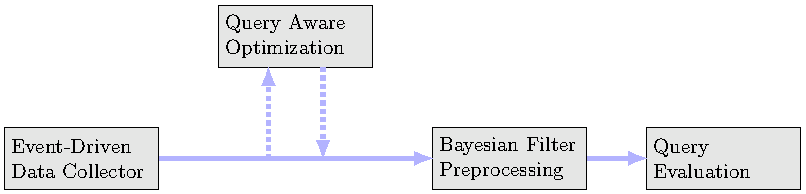
\includegraphics[width=.8\textwidth]{img/system-design.pdf}
\caption{\label{fig:overall}
Overall system structure}
\end{figure}

Figure \ref{fig:overall} shows the overall structure of our system design.
Raw readings are first fed into and processed by the event-driven
raw data collector module, which then provides aggregated readings
for each object at every second to the Bayesian filtering-based
preprocessing module.  Before running the preprocessing module, the
reading data may be optionally sent to the query aware optimization
module which filters out non-candidate objects according to
registered queries and objects' most recent readings, and outputs a
candidate set \(C\) to the Bayesian filtering-based preprocessing
module.  The preprocessing module cleanses noisy raw data for each
object in \(C\), stores the resulting probabilistic data in a hash
table, and passes the hash table to the query evaluation module.  At
last, the query evaluation module answers registered queries based
on the hash table that contains filtered data.

\chapter{Event-Driven Raw Data Collector}
\label{sec:data-collector}
In this subsection, we describe the event-driven raw data collector
which is the front end of the entire system. The data collector
module is responsible for storing RFID raw readings in an efficient
way for the following query processing tasks.  Considering the
characteristics of Bayesian filtering, readings of one detecting
device alone cannot effectively infer an object's moving direction
and speed, while readings of two or more detecting devices can. We
define events in this context as the object either entering (ENTER
event) or leaving (LEAVE event) the reading range of an RFID
reader. To minimize the storage space for every object, the data
collector module only stores readings during the most recent
\{ENTER, LEAVE, ENTER\} events, and removes earlier readings. In
other words, our system only stores readings of up to the two most
recent consecutive detecting devices for every object. For example,
if an object is previously identified by \(d_i\) and \(d_j\),
readings from \(d_i\) and \(d_j\) are stored in the data
collector. When the object is entering the detection range of a new
device \(d_k\), the data collector will record readings from
\(d_k\) while removing older readings from \(d_i\). The previous
readings have negligible effects on the current prediction.

The data collector module is also responsible for aggregating the
raw readings to more concise entries with a time unit of one
second. RFID readers usually have a high reading rate of tens of
samples per second.  However, Bayesian filtering does not need such
a high observation frequency.  An update frequency of once per
second would provide a good enough resolution.  Therefore,
aggregation of the raw readings can further save storage without
compromising accuracy.

\chapter{Indoor Walking Graph Model and Anchor Point Indexing Model}
\label{sec:walking-graph-anchor-point}
This subsection introduces the underlying assumptions and backbone
models of our system, which forms the basis for understanding
subsequent sections.  We propose two novel models in our system,
indoor walking graph model and anchor point indexing model, for
tracking object locations in indoor environments.

\section{Indoor Walking Graph Model}
\label{sec:org1b9f4d5}

we assume our system setting is a typical office building where
the width of hallways can be fully covered by the detection range
of sensing devices (which is usually true since the detection
range of RFID readers can be as long as 3 meters), and RFID
readers are deployed only along the hallways.  In this case the
hallways can simply be modeled as lines, since from RFID reading
results alone, the locations along the width of hallways cannot be
inferred.  Furthermore, since no RFID readers are deployed inside
rooms, the resolution of location inferences cannot be higher than
a single room.

\begin{figure}[htbp]
\centering
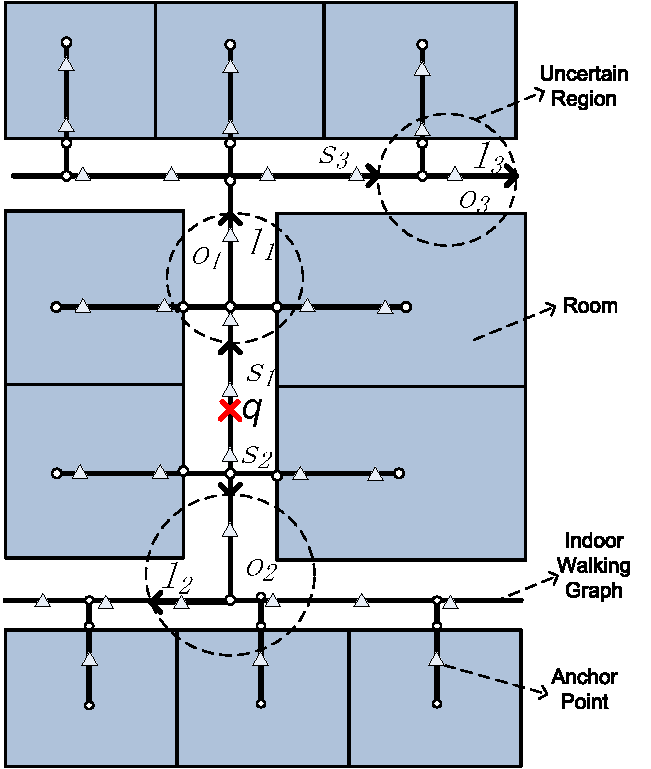
\includegraphics[width=.5\textwidth]{img/knn-filter-non-candidates.pdf}
\caption{\label{fig:knn-filter-non-candidates}
Example of filtering out \(k\)NN query non-candidate objects.}
\end{figure}

Based on the above assumptions, we propose an \emph{indoor walking
graph model}.  The indoor walking graph \(G\langle N, E\rangle\)
is abstracted from the regular walking patterns of people in an
indoor environment, and can represent any accessible path in the
environment.  The graph \(G\) comprises a set \(N\) of nodes
(i.e., intersections) together with a set \(E\) of edges (i.e.,
hallways).  By restricting object movements to be only on the
edges \(E\) of \(G\), we can greatly simplify the object movement
model while at the same time still preserving the inference
accuracy of Bayesian filtering.  Also, the distance metric used in
this paper, e.g., in \(k\)NN query evaluations, can simply be the
shortest spatial network distance on \(G\), which can then be
calculated by many well-known spatial network shortest path
algorithms \cite{papadias2003-query,samet2008-scalable}, as shown in
Figure \ref{fig:knn-filter-non-candidates}.

\section{Anchor Point Indexing Model}
\label{sec:org46e33c2}

the indoor walking graph edges \(E\) are by nature continuous.  To
simplify the representation of an object's location distribution
on \(E\), we propose an effective spatial indexing method: anchor
point-based indexing.  We define anchor points as a set \(AP\) of
predefined points on \(E\) with a uniform distance (such as 1
meter) to each other.  An example of anchor points is shown in
Figure \ref{fig:knn-filter-non-candidates}.  In essence, the model of
anchor points is a scheme of trying to discretize objects'
locations.  After Bayesian filtering is finished for an object
\(o_i\), its location probability distribution is aggregated to
discrete anchor points.  Specifically, for the Kalman filter, an
integration of an object's bell-shaped location distribution
between two adjacent anchor points is calculated. For particle
filters, suppose \(ap_j\) is an anchor point with a nonzero number
\(n\) of particles, \(p_i(o_i.location=ap_j)=n/N_s\), where
\(p_i\) is the probability distribution function that \(o_i\) is
at \(ap_j\) and \(N_s\) is the total number of particles for
\(o_i\).

A hash table \texttt{APtoObjHT} is maintained in our system with the key
to be the coordinates of an anchor point \(ap_j\) and returned
value the list of each object and its probability at the anchor
point \(\langle o_i, p_i(ap_j)\rangle\).  For instance, an entry
of \texttt{APtoObjHT} would look like: \((8.5, 6.2), \{\langle o_1,
    0.14\rangle, \langle o_3, 0.03\rangle, \langle o_7, 0.37\rangle
    \}\), which means at the anchor point with coordinate (8.5, 6.2),
there are three possible objects \(o_1\), \(o_3\), and \(o_7\),
with probabilities of 0.14, 0.03, and 0.37, respectively.  With
the help of the above anchor point indexing model, the query
evaluation module can simply refer to the hash table \texttt{APtoObjHT}
to determine objects' location distributions.

\chapter{Query Aware Optimization Module}
\label{sec:optimization-module}
To answer every range query or \(k\)NN query, a naive approach is
to calculate the probability distribution of every object's
location currently in the indoor setting.  However, if query ranges
cover only a small fraction of the whole area, then there will be a
considerable percentage of objects who are guaranteed to not be in
the result set of any query.  We call those objects that have no
chance to be in any result set "non-candidate objects".  The
computational cost of running Bayesian filters for non-candidate
objects should be saved.  In this subsection we present two
efficient methods to filter out non-candidate objects for range
query and \(k\)NN query, respectively.

\section{Range Query}
\label{sec:range-query}
To decrease the computational cost, we employ a simple approach
based on the Euclidian distance instead of the minimum indoor
walking distance \cite{yang2010-probabilistic} to filter out
non-candidate objects.  An example of the optimization process is
shown in Figure \ref{fig:range-filter-non-candidates}.  For every object
\(o_i\), its most recent detecting device \(d\) and last reading
time stamp \(t_{last}\) are first retrieved from the data
collector module.  We assume the maximum walking speed of people
to be \(u_{max}\).  Within the time period from \(t_{last}\) to
the present time \(t_{current}\), the maximum walking distance of
a person is \(l_{max}=u_{max}*(t_{current}-t_{last})\).  We define
\(o_i\)'s uncertain region \(UR(o_i)\) to be a circle centered at
\(d\) with radius \(r=l_{max}+d.range\).  If \(UR(o_i)\) does not
overlap with any query range then \(o_i\) is not a candidate and
should be filtered out.  On the contrary, if \(UR(o_i)\) overlaps
with one or more query ranges then we add \(o_i\) to the result
candidate set \(C\).  In Figure \ref{fig:range-filter-non-candidates},
the only object in the figure should be filtered out since its
uncertain region does not intersect with any range query currently
evaluated in the system.

\begin{figure}[htbp]
\centering
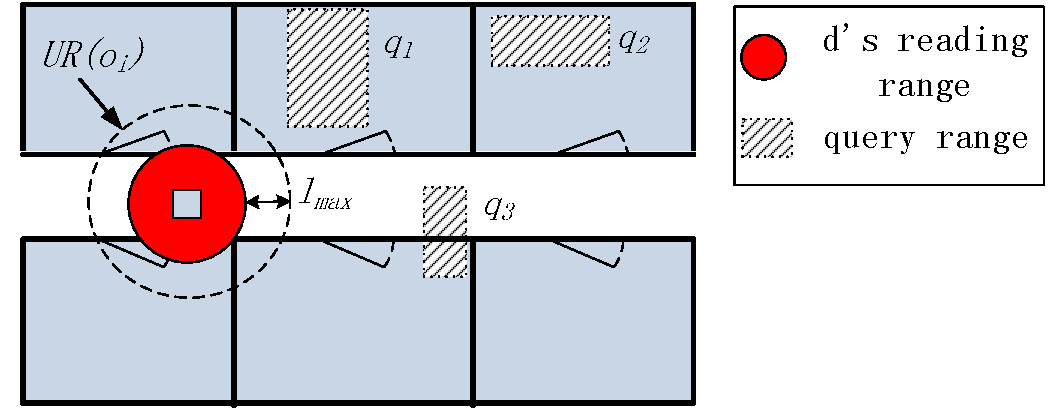
\includegraphics[width=.7\textwidth]{img/range-filter-non-candidates.pdf}
\caption{\label{fig:range-filter-non-candidates}
Example of filtering out range query non-candidate objects.}
\end{figure}

\section{\(k\)NN Query}
\label{sec:knn-query}
By employing the idea of distance-based pruning in
\cite{yang2009-scalable}, we perform a similar distance pruning for
\(k\)NN queries to identify candidate objects.  We use \(s_i
    (l_i)\) to denote the minimum (maximum) shortest network distance
(with respect to the indoor walking graph) from a given query
point \(q\) to the uncertain region of \(o_i\):
\begin{equation}
  \begin{split}
    s_i &= \min_{p\in UR(o_i)} d_{shortestpath}(q, p)\\
    l_i &= \max_{p\in UR(o_i)} d_{shortestpath}(q, p)
  \end{split}
\end{equation}

Let \(f\) be the \(k^{th}\) minimum of all objects' \(l_i\)
values.  If \(s_i\) of object \(o_i\) is greater than \(f\),
object \(o_i\) can be safely pruned since there exist at least
\(k\) objects whose entire uncertain regions are definitely closer
to \(q\) than \(o_i\)'s shortest possible distance to \(q\).
Figure \ref{fig:knn-filter-non-candidates} is an example pruning process
for a 2NN query: There are 3 objects in total in the system.  We
can see \(l_1<l_2<l_3\) and consequently \(f=l_2\) in this case;
\(s_3\) is greater than \(f\), so \(o_3\) has no chance to be in
the result set of the 2NN query.  We run the distance pruning for
every \(k\)NN query and add possible candidate objects to \(C\).

Finally, a candidate set \(C\) is produced by this module,
containing objects that might be in the result set of one or more
range queries or \(k\)NN queries.  \(C\) is then fed into the
Bayesian filtering-based preprocessing module which will be
explained in the next subsection.

\chapter{Bayesian Filtering-based Preprocessing Module}
\label{sec:preprocessing-module}
The preprocessing module estimates an object's location
distribution according to its two most recent readings, calculates
the discrete probability on anchor points, and stores the results
to the hash table \texttt{APtoObjHT}.  We introduce two preprocessing
approaches based on two famous algorithms in the Bayesian Filtering
family: the \emph{Kalman filter} and the \emph{Particle filter}.

\section{Kalman Filter-Based Preprocessing Module}
\label{sec:kalman-filter-preprocessing}
In this section, we extend the basic 1-D example of the Kalman
filter in Section \ref{sec:kalman-filter} to be suitable for more
complex 2D indoor settings.  Due to the irregularity of indoor
layout, the main challenge here is that an object's moving path
may diverge to multiple paths.  For example, in Figure
\ref{fig:kalman-filter}, assume that an object was detected first by
reader \(d_1\) at \(t_1\) then by reader \(d_2\) at \(t_2\), it
could have entered \(R_2\) or \(R_6\) before proceeding to
\(d_2\).  When we conduct a prediction with the Kalman filter, we
need to consider all possible paths, each of which will give a
separate prediction.  Algorithm \ref{alg:kalman-filter} formulates
our approach of applying the Kalman filter to estimate objects'
locations, which is elaborated in the rest of this subsection with
the example in Figure \ref{fig:kalman-filter}.

\begin{figure}[htbp]
\centering
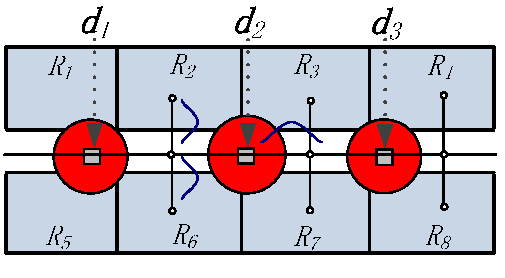
\includegraphics[width=.5\textwidth]{img/kalman-example.pdf}
\caption{\label{fig:kalman-filter}
Example of Kalman filter-based prediction.}
\end{figure}

The Kalman filter algorithm starts by first retrieving most recent
readings for each candidate from the data collector module.  Line
5 of Algorithm \ref{alg:kalman-filter} restricts the Kalman filter
from running more than 60 seconds beyond the last active reading,
otherwise its location estimation will become dispersed over too
large a area and the filtering result will become unusable.

We assume objects' speed \(v\) is a Gaussian variable with mean
\(\mu=1\) m/s and variance \(\sigma=0.1\), and the time of an
object staying inside a room \(t_{room}\) also follows Gaussian
distribution.  From line 6 to 11, we assume that objects rarely
enter the same room more than once.  Suppose there are \(m\) rooms
from \(d_1\) to \(d_2\), then there are \(m+1\) different
predictions \(\hat{x}_{2^-} = \hat{x}_1 + v * (t_2 - t_1-i *
    \mu_{t_{room}})\) where \(i=0,\ldots,m\) represents the number of
rooms the object entered during \(t_1\) to \(t_2\).  Note that we
simplify \(\hat{x}_{2^-}\) by replacing \(t_{room}\) with its mean
value \(\mu_{t_{room}}\).

When the observation at \(t_2\) is made, we combine the
observation with only reasonable predictions to get a final
estimation. By "reasonable", we mean predictions with a good
portion of pdf overlapping with \(d_2\)'s reading range.  For
example, in Figure \ref{fig:kalman-filter}, the two predictions for the
two paths entering \(R_2\) and \(R_6\) respectively are hardly
overlapping with \(d_2\)'s reading range, so we can safely prune
them and only consider the rightmost prediction.  After pruning,
the average of remaining predictions is used to calculate the
object's location estimation at \(t_2\) according to Equations
\eqref{eq:kalmanmean} and \eqref{eq:kalmanvar}.

From the latest detected time \(t_2\) to current, the object can
take every possible path from \(d_2\) going forward.  Line 15 uses
recursion to enumerate all the possibilities and line 16
calculates the probability distribution of \(\hat{x}_{min^-}\) by
counting the number of cases of the object in a particular room or
at a particular location along the hallway divided by the total
number of cases.  At last, from line 18 to 21, we calculate the
integration of the object's location probability distribution
function from the current anchor point to its adjacent point, and
store the discrete probability of the object's location being on a
certain anchor point to \texttt{APtoObjHT}.
\begin{algorithm}[!t]
  \caption{Kalman Filter(\(C\))}
  \label{alg:kalman-filter}
  \small
  \begin{algorithmic}[1]
    \FOR {each object \(o_i\) of \(C\)}
    \STATE retrieve \(o_i\)'s aggregated readings from the data collector module
    \STATE \(t_1\), \(t_2\) = the starting/ending time of the aggregated readings
    \STATE \(d_1\), \(d_2\) = the second most/most recent detecting devices for \(o_i\)
    \STATE \(t_{min}\) = min(\(t_2+60, t_{current}\))
    \STATE \(m\) = number of rooms from \(d_1\) to \(d_2\)
    \FOR {\(i=0,\ldots,m\)}
    \STATE \(\hat{x}_{2^-}=\hat{x}_1+v*(t_2-t_1-i*\mu_{t_{room}})\)
    \STATE \(\sigma_{2^-}^2=\sigma_1^2+\sigma_v^2*(t_2-t_1)\)
    \STATE prune if this distribution's overlap with \(d_2\)'s range is below threshold
    \ENDFOR
    \STATE average all the predictions
    \STATE calculate \(\hat{x}_2\) and \(\sigma_2^2\) by employing Equations~\ref{eq:kalmanmean} and~\ref{eq:kalmanvar}
    \STATE recursively enumerate all possible paths from \(\hat{x}_2\) going forward until \(t_{min}\)
    \STATE estimate \(o_i\)'s location \(\hat{x}_{min^-}\) by counting
    \STATE \(\sigma_{min^-}^2=\sigma_2^2+\sigma_v^2*(t_{min}-t_2)\)
    \FOR {each anchor point \(ap_j\) with a nontrivial probability under estimated location distribution}
    \STATE calculate probability \(p_i(o_i.location=ap_j)\)
    \STATE update Hash Table \texttt{APtoObjHT}
    \ENDFOR
    \ENDFOR
  \end{algorithmic}
\end{algorithm}

\section{Particle Filter-Based Preprocessing Module}
\label{sec:particle-filter-preprocessing}
\begin{algorithm}[!t]
  \algsetup{linenosize=\small,linenodelimiter=.}
  \caption{Particle Filter(\(C\))}
  \label{alg:particle-filter}
  \small
  \begin{algorithmic}[1]
    \FOR {each object \(o_i\) of \(C\)}
    \STATE retrieve \(o_i\)'s aggregated readings from the data collector module
    \STATE \(t_1\), \(t_2\) = the starting/ending time of the aggregated readings
    \STATE \(d_1\), \(d_2\) = the second most/most recent detecting devices for \(o_i\)
    \STATE initialize particles with random speed and direction within \(d_2.activationRange\)
    \STATE \(t_{min}\) = min(\(t_2+60, t_{current}\))
    \FOR {every second \(t_j\) from \(t_1\) to \(t_{min}\)}
    \FOR {every particle \(p_m\) of \(o_i\)}
    \STATE \(p_m\) updates its location
    \ENDFOR
    \STATE retrieve the aggregated reading entry \emph{reading} of \(t_j\)
    \IF {\(reading.Device\)=\emph{null}}
    \STATE continue
    \ELSE
    \FOR {every particle \(p_m\) of \(o_i\)}
    \STATE update \(p_m\)'s weight
    \ENDFOR
    \STATE normalize the weights of all particles of \(o_i\)
    \STATE Resampling() %// Algorithm~\ref{alg:RS}
    \ENDIF
    \ENDFOR
    \STATE assign particles of \(o_i\) to their nearest anchor points
    \FOR {each anchor point \(ap_j\) with a nonzero number of particles \(n\)}
    \STATE calculate probability \(p_i(o_i.location=ap_j)=n/N_s\)
    \STATE update Hash Table \texttt{APtoObjHT}
    \ENDFOR
    \ENDFOR
  \end{algorithmic}
\end{algorithm}

The particle filter method consists of 3 steps: initialization,
particle updating, and particle resampling.  In the first step, a
set of particles are generated and uniformly distributed on the
graph edges within the detection range of \(d_2\), and each
particle picks its own moving direction and speed as in line 5.
In our system, particles' speeds are drawn from a Gaussian
distribution with mean \(\mu=1\) m/s and \(\sigma=0.1\).  In the
location updating step in line 9, particles move along graph edges
according to their speed and direction, and will pick a random
direction at intersections; if particles are inside rooms, they
continue to stay inside with probability 0.9 and move out with
probability 0.1.  After location updating, in line 16 particles'
weights are updated according to their consistency with reading
results.  In other words, particles within the detecting device's
range are assigned a high weight, while others are assigned a low
weight.  In the resampling step, particles' weights are first
normalized as in line 18.  We then employ the Resampling Algorithm
\cite{yu2013-rfid} to replicate highly weighted particles and remove
lowly weighted particles as in line 19.  Lines 23 to 26 discretize
the filtered probabilistic data and build the hash table
\texttt{APtoObjHT} as described in Section
\ref{sec:walking-graph-anchor-point}.

\chapter{Query Evaluation}
\label{sec:query-evaluation}
In this subsection we are going to discuss how to evaluate range
and \(k\)NN queries efficiently with the filtered probabilistic
data in the hash table \texttt{APtoObjHT}.  For \(k\)NN queries, without
loss of generality, the query point is approximated to the nearest
edge of the indoor walking graph for simplicity.

\section{Indoor Range Query}
\label{sec:org4ae245f}

To evaluate indoor range queries, the first thought would be to
determine the anchor points within the range, then answer the
query by returning objects and their associated probabilities
indexed by those anchor points.  However, with further
consideration, we can see that since anchor points are restricted
to be only on graph edges, they are actually the 1D projection of
2D spaces; the loss of one dimension should be compensated in the
query evaluation process.  Figure \ref{fig:range-query} shows an example
of how the compensation is done with respect to two different
types of indoor entities: hallways and rooms.

\begin{figure}[htbp]
\centering
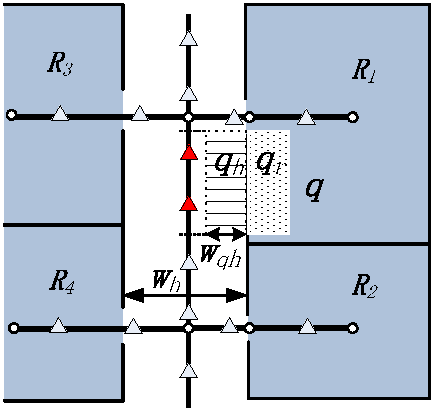
\includegraphics[width=.5\textwidth]{img/range-query.pdf}
\caption{\label{fig:range-query}
Example of indoor range query.}
\end{figure}

In Figure \ref{fig:range-query}, query \(q\) is a rectangle which
intersects with both the hallway and room \(R_1\), but does not
directly contain any anchor point.  We denote the left part of
\(q\) which overlaps with the hallway as \(q_h\), and the right
part which overlaps with \(R_1\) as \(q_r\).  We first look at how
to evaluate the hallway part of \(q\).  The anchor points which
fall within \(q\)'s vertical range are marked red in Figure
\ref{fig:range-query}, and should be considered for answering \(q_h\).
Since in our assumptions no differentiation along the width of
hallways can be inferred about an object's true location, objects
in hallways can be anywhere along the width of hallways with equal
probability.  With this assumption, the ratio of \(w_{q_h}\) (the
width of \(q_h\)) and \(w_h\) (the width of the hallway) will
indicate the probability of objects in hallways within the
vertical range of \(q\) being in \(q_h\).  For example, if an
object \(o_i\) is in the hallway and in the vertical range of
\(q\) with probability \(p_1\), which can be calculated by summing
up the probabilities indexed by the red anchor points, then the
probability of this object being in \(q_h\) is
\(p_i(o_i.location\in q_h)=p_1*w_{q_h}/w_h\).

Then we look at the room part of \(q\).  The anchor points within
room \(R_1\) should represent the whole 2D area of \(R_1\), and
again we assume objects inside rooms are uniformly distributed.
Similar to the hallway situation, the ratio of \(q_r\)'s area to
\(R_1\)'s area is the probability of an object in \(R_1\)
happening to be in \(q_r\).  For example, if \(o_i\)'s probability
of being in \(R_1\) is \(p_2\), then its probability of being in
\(q_r\) is \(p_i(o_i.location\in q_r)=p_2*Area_{q_r}/Area_{R_1}\),
where \(p_2\) can be calculated by summing up the indexed
probabilities of \(o_i\) on all the anchor points inside \(R_1\)
and \(Area_i\) stands for the size of a given region \(i\).

\begin{algorithm}[!t]
  \algsetup{linenosize=\small,linenodelimiter=.}
  \caption{Indoor Range Query(\(q\))}
  \label{alg:range-query}
  \small
  \begin{algorithmic}[1]
    \STATE resultSet=\(\emptyset\) \STATE cells=getIntersect(\(q\)) \FOR
    {every cell in cells}
    \IF{cell.type=HALLWAY}
    \STATE anchorpoints=cell.getCoveredAP(\(q\))
    \STATE ratio=cell.getWidthRatio(\(q\))
    \ELSIF{cell.type=ROOM}
    \STATE anchorpoints=cell.getInsideAP()
    \STATE ratio=cell.getAreaRatio(\(q\))
    \ENDIF
    \STATE result=\(\emptyset\)
    \FOR{each ap in anchorpoints}
    \STATE result=result+APtoObjHT.get(\(ap\))
    \ENDFOR
    \STATE result=result*ratio
    \STATE resultSet=resultSet+result
    \ENDFOR \RETURN resultSet
  \end{algorithmic}
\end{algorithm}

Algorithm \ref{alg:range-query} summarizes the above procedures.  In
line 15, we define the multiply operation for \texttt{resultSet} to
adjust the probabilities for all objects in it by the multiplying
constant.  In line 16, we define the addition operation for
\texttt{resultSet} to be: if an object probability pair \(\langle o_i,
    p\rangle\) is to be added, we check whether \(o_i\) already exists
in \texttt{resultSet}.  If so, we just add \(p\) to the probability of
\(o_i\) in \texttt{resultSet}; otherwise, we insert \(\langle o_i,
    p\rangle\) to \texttt{resultSet}.  For instance, suppose \texttt{resultSet}
originally contains \(\{(o_1, 0.2), (o_2, 0.15)\}\), and result
stores \(\{(o_2, 0.1), (o_3, 0.05)\}\).  \texttt{resultSet} is updated to
be \(\{(o_1, 0.2), (o_2, 0.25), (o_3, 0.05)\}\) after the addition
in line 16.

\section{Indoor \(k\)NN Query}
\label{sec:org603decf}

For indoor \(k\)NN queries, we present an efficient evaluation
method with statistical accuracy.  Unlike previous work
\cite{yang2010-probabilistic,cheng2009-evaluating}, which involves
heavy computation and returns multiple result sets for users to
choose, our method is user friendly and returns a relatively small
number of candidate objects.  Our method works as follows:
starting from the query point \(q\), anchor points are searched in
ascending order of their distance to \(q\); the search expands
from \(q\) one achor point forward per iteration, until the sum of
the probability of all objects indexed by the searched anchor
points is no less than \(k\).  The result set has the form of
\(\langle(o_1, p_1), (o_2, p_2), \ldots, (o_m, p_m)\rangle\) where
\(\sum_{i=1}^{m} p_i \geq k\).  The number of returned objects
will be at least \(k\).  From the sense of statistics, the
probability \(p_i\) associated with object \(o_i\) in the result
set is the probability of \(o_i\) being in the \(k\)NN result set
of \(q\).  The algorithm of the indoor \(k\)NN query evaluation
method in our work is shown in Algorithm \ref{alg:knn}.
\begin{algorithm}[!t]
  \algsetup{linenosize=\small,linenodelimiter=.}
  \caption{Indoor \(k\)NN Query(\(q\), \(k\))}
  \label{alg:knn}
  \small
  \begin{algorithmic}[1]
    \STATE resultSet=\(\emptyset\)
    \STATE \(\overline{n_in_j}\)=find\_segment(\(q\))
    \STATE vector V=\(\langle(n_i,q), (n_j,q)\rangle\)  // elements in V have the form (node, prevNode) \FOR {every entry \(e\) in V}
    \STATE anchorpoint=find\_nextAnchorPoint(\(e\)) // return the next unsearched anchor point from \(e\).prevNode to \(e\).node
    \IF{anchorpoint=\(\emptyset\)}
    \STATE remove \(e\) from \(V\)
    \FOR{each unvisited adjacent node \(n_x\) of \(e\).node}
    \STATE add (\(n_x\), \(e\).node) to V
    \ENDFOR
    \STATE continue
    \ENDIF
    \STATE resultSet=resultSet+APtoObjHT.get(anchorpoint)
    \STATE \(prob_{total}\)=resultSet.getTotalProb() %//calculate the probability sum of all objects in resultSet
    \IF{\(prob_{total} >= k\)}
    \STATE break
    \ENDIF
    \ENDFOR \RETURN resultSet
  \end{algorithmic}
\end{algorithm}

In Algorithm \ref{alg:knn}, lines 1 and 2 are initial setups.  Line
3 adds two entries to a vector \(V\), whose elements store the
edge segments expanding out from query point \(q\).  In the
following for loop, line 5 finds the next unvisited anchor point
further away from \(q\).  If all anchor points are already
searched on an edge segment \(e\), lines 6 to 12 remove \(e\) and
add all adjacent unvisited edges of \(e\).node to \(V\).  Line 13
updates the result set by adding \(\langle\)object ID,
probability\(\rangle\) pairs indexed by the current anchor point
to it.  In lines 14 to 17, the total probability of all objects in
the result set is checked, and if it equals or exceeds \(k\), the
algorithm ends and returns the result set.  Note that the stopping
criteria of our \(k\)NN algorithm do not require emptying the
frontier edges in \(V\).

\begin{figure}[htbp]
\centering
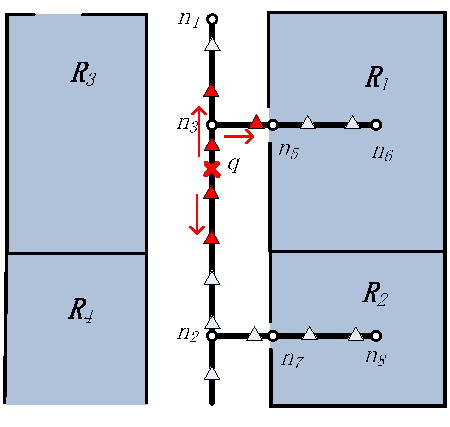
\includegraphics[width=.5\textwidth]{img/knn.pdf}
\caption{\label{fig:knn}
Example of indoor \(k\)NN query.}
\end{figure}

An example \(k\)NN query is shown in Figure \ref{fig:knn}, which is a
snapshot of the running status of Algorithm \ref{alg:knn}.  In Figure
\ref{fig:knn}, red arrows indicate the searching directions expanding
from \(q\), and red anchor points indicate the points that have
already been searched.  Note that the edge segment from \(q\) to
\(n_3\) is already removed from \(V\) and new edges
\(\overline{n_3n_4}\), \(\overline{n_3n_5}\) are currently in
\(V\) as well as \(\overline{n_2q}\).  The search process is to be
continued until the total probability of the result set is no less
than \(k\).

\section{Continuous Indoor Range Query}
\label{sec:org1bac622}

In this subsection, we aim to solve the problem of continuous
indoor range query on filtered probabilistic data.  To efficiently
monitor the result set, we use a similar concept \emph{critical device}
as in \cite{yang2009-scalable}, which can save considerable
computations rather than constantly repeating the snapshot
algorithm.  We define \emph{critical devices} for a query to be only
the set of devices whose readings will affect the query results.
Our continuous monitoring algorithm is distinct from Yang's work
\cite{yang2009-scalable} in two aspects: first, we leverage the
Indoor Walking Graph to simplify the identification process of
critical devices; second, the probability updating process is
Bayesian filter-based, which is more accurate and very different
from Yang's approach in nature.

To identify critical devices for a range query, we propose an
approach consisting of two steps, mapping and searching.  For the
mapping step, we categorize two different cases:

\begin{description}
\item[{Case 1}] the whole query range is contained within one room or
adjacent rooms, then we project from the doors of end rooms
to \(E\) along hallways.  For example, \(q_1\) in Figure
\ref{fig:critical-device} is fully contained in room \(R_1\), so it
is projected to a point (the red point) on \(E\) through the
door of \(R_1\).
\item[{Case 2}] the query range overlaps with both rooms and hallways,
then the endpoints of mapped edge segment(s) should take
whichever makes the covered segment longer among projected
points of query range ends and end rooms' doors.  \(q_2\) in
Figure \ref{fig:critical-device} is an example of this case.  It is
mapped to an edge segment, \(\overline{ab}\), along the
hallway as marked in red.  Point \(a\), room \(R_1\) door's
projected point, is chosen instead of \(c\), the query range
end projected point.  Similarly, point \(b\) is chosen
instead of \(d\).
\end{description}

For the searching step, an expansion starting from the mapped
endpoint(s) is performed along \(E\) until the activation range of
an RFID reader or deadend is reached.

\begin{figure}[htbp]
\centering
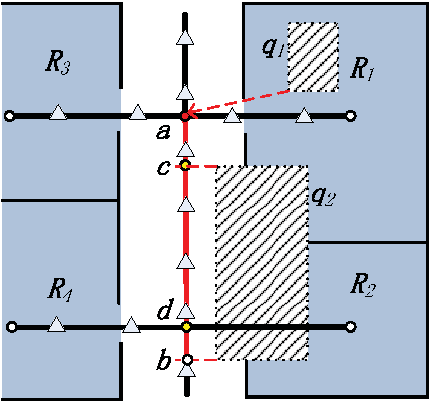
\includegraphics[width=.5\textwidth]{img/critical-device.pdf}
\caption{\label{fig:critical-device}
Mapping process to identify critical devices.}
\end{figure}

For the initial evaluation of a query, we change the optimization
algorithm in Section \ref{sec:optimization-module} of the snapshot
query to fully take advantage of critical devices.  For an object
to be in the query range, it must be most recently detected by a
critical device or any device that is bounded by the critical
devices.  Other than the difference in identifying the candidate
object set, other parts of the initial evaluation algorithm are
the same as its snapshot counterpart.  After initial evaluation,
we continuously monitor the candidate set by performing Bayesian
filters for them at every time step.

During the lifetime of a query, the candidate set may change due
to candidates moving out or non-candidates moving into the
critical device bounded region.  If a candidate object is detected
by a critical device, or the object's probability of still
residing in the bounded region falls to 0, then we assume that it
is moving out and should be removed from the candidate set.  On
the other hand, if a non-candidate object enters the detection
range of a critical device, we assume it is moving into the
bounded region and should be added to the candidate set.

The proposed continuous indoor range query is formalized in
Algorithm \ref{alg:continuous-range-query}.  Lines 1 to 6 initialize
the critical devices and candidate set for query \(q\).  In line 4
we use a new hash table \texttt{DtoObj}, which maps a device to objects
whose most recent readings are from this device.  Lines 9 to 20
update the candidate set according to the readings of critical
devices, and also objects' probabilities of presence within the
bounded region.  Line 21 executes Algorithms \ref{alg:kalman-filter}
or \ref{alg:particle-filter} to update candidate objects' location
distribution probabilities.  Line 22 calculates the result set
using Algorithm \ref{alg:range-query}.  Note that for Algorithm
\ref{alg:range-query} there is no need to recompute anchor point set
since it remains unchanged until the query is unregistered from
the system.

\begin{algorithm}[!t]
  \algsetup{linenosize=\small,linenodelimiter=.}
  \caption{Continuous Range Query(\(q\))}
  \label{alg:continuous-range-query}
  \small
  \begin{algorithmic}[1]
    \STATE \(D_{cd}=getCriticalDevices(q)\) \STATE \(C=\emptyset\)
    \FOR{every \(reader\) in or bounded by \(D_{cd}\)}
    \STATE \(C=C\bigcup DtoObj(reader)\)
    \ENDFOR \STATE Bayesian Filter(\(C\)) \STATE \(R_{init}\)=Indoor Range
    Query(\(q\))
    \FOR{every time step from \(t_{reg}\) to \(t_{unreg}\)}
    \FOR{every \(o_i\) detected by any reader in \(D_{cd}\)}
    \IF{\(o_i\in C\)}
    \STATE \(C\).remove(\(o_i\))
    \ELSE
    \STATE \(C\).add(\(o_i\))
    \ENDIF
    \ENDFOR
    \FOR{every \(o_i \in C\)}
    \IF{\(p(o_i.location \in bounded region of D_{cd})=0\)}
    \STATE \(C\).remove(\(o_i\))
    \ENDIF
    \ENDFOR
    \STATE Bayesian Filter(\(C\))
    \STATE \(R\)=Indoor Range Query(\(q\))
    \ENDFOR
  \end{algorithmic}
\end{algorithm}

\section{Continuous Indoor \(k\)NN Query}
\label{sec:orgae0624e}

Similar to continuous indoor range query, how to update the
candidate set of continuous indoor \(k\)NN query is crucial.  To
reduce the overhead of computing the candidate set at every time
step, we buffer a certain number of extra candidates, and only
recompute the candidate set according to the optimization approach
in Section \ref{sec:optimization-module} when the total number of
candidates is less than \(k\).

Recall from Section \ref{sec:optimization-module}, by examining the
minimum (\(s_i\))/maximum (\(l_i\)) shortest network distance from
the query point \(q\) to an object's uncertain region, the
snapshot optimization approach excludes objects with \(s_i>f\).
Note that the candidate set identified by this method contains at
least \(k\) objects (usually more than \(k\)).  Based on this
snapshot optimization approach, we extend it to include at least
\(k+y\) candidates where \(y\) is a user configurable parameter.
Obviously, \(y\) represents a tradeoff between the size of
candidate set and the recomputation frequency.  We accomplish this
by calculating the \((k+y)\)-th minimum \(l_i\) among all objects,
and use this value as a threshold to cut off non-candidate
objects.

During continuous monitoring, we need to make sure that the
candidate set gets updated accordingly when objects move away or
towards \(q\).  We still use critical devices to monitor
candidates, but now the critical devices may change each time the
candidate set is recomputed.  The identification process of
critical devices goes like the following: after calculating the
candidate set, a search is performed from \(q\) along \(E\) to
cover all the uncertain regions of candidate objects, until
reaching readers (critical devices) or deadend.  As we can see,
critical devices form a bounded region where at least \(k+y\)
candidate objects are for sure inside it.

The proposed continuous indoor \(k\)NN query is formalized in
Algorithm \ref{alg:continuous-knn}.  Note that in lines 13 to 16,
when the total number of candidates falls below \(k\), we need to
recompute a new candidate set of at least \(k+y\) objects, and
identify new critical devices accordingly.

\begin{algorithm}[!t]
  \algsetup{linenosize=\small,linenodelimiter=.}
  \caption{Continuous \(k\)NN Query(\(q\), \(k\), \(y\))}
  \label{alg:continuous-knn}
  \small
  \begin{algorithmic}[1]
    \STATE \(C=getCandidateObjects(k+y)\) \STATE
    \(D_{cd}=getCriticalDevices(C)\) \STATE Bayesian Filter(\(C\)) \STATE
    \(R_{init}\)=Indoor \(k\)NN Query(\(q\), \(k\))
    \FOR{every time step from \(t_{reg}\) to \(t_{unreg}\)}
    \FOR{every \(o_i\) detected by any reader in \(D_{cd}\)}
    \IF{\(o_i\in C\)}
    \STATE \(C\).remove(\(o_i\))
    \ELSE
    \STATE \(C\).add(\(o_i\))
    \ENDIF
    \ENDFOR
    \IF{\(C.count<k\)}
    \STATE \(C=getCandidateObjects(k+y)\)
    \STATE \(D_{cd}=getCriticalDevices(C)\)
    \ENDIF
    \STATE Bayesian Filter(\(C\))
    \STATE \(R\)=Indoor \(k\)NN Query(\(q\), \(k\))
    \ENDFOR
  \end{algorithmic}
\end{algorithm}

\part{Experiment}
\label{sec:experiment}
In this section, we evaluate the performance of the proposed
Bayesian filtering-based indoor spatial query evaluation system
using the data generated by real-world parameters and compare the
results with the symbolic model-based solution
\cite{yang2010-probabilistic}.  The proposed algorithms are
implemented in \texttt{C++}.  All the experiments were conducted on an
Ubuntu Linux server equipped with an Intel Xeon 2.4GHz processor and
16GB memory.  In our experiments, the floor plan, which is of the
second floor of the Haley Center on Auburn University campus,
includes 30 rooms and 4 hallways on a single floor, in which all
rooms are connected to one or more hallways by doors.  A total of 19
RFID readers are deployed on hallways with uniform distance to each
other.

\chapter{Simulator Implementation}
\label{sec:orgcaf1209}

\begin{figure}[htbp]
\centering
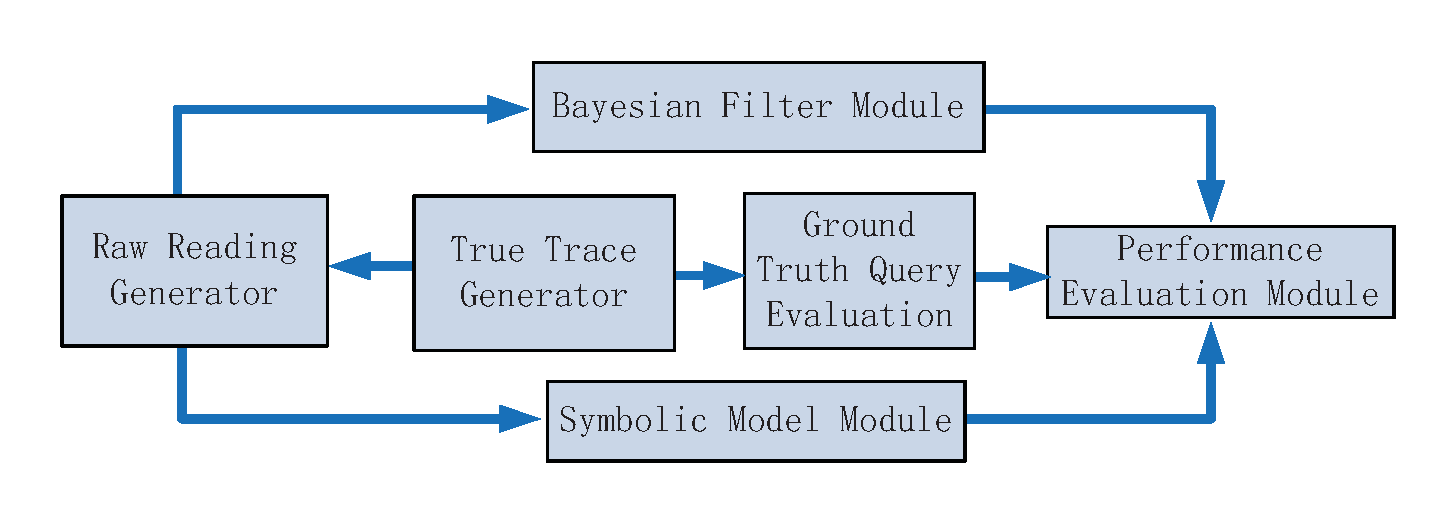
\includegraphics[width=.8\textwidth]{img/simulator-structure.pdf}
\caption{\label{fig:simulator-structure}
The simulator structure.}
\end{figure}

The whole simulator consists of six components, including true
trace generator, raw reading generator, Bayesian filter module,
symbolic model module, ground truth query evaluation, and
performance evaluation module.  Figure \ref{fig:simulator-structure}
shows the relationship of different components in the simulation
system.  The true trace generator module is responsible for
generating the ground truth traces of moving objects and recording
the true location of each object every second.  Each object
randomly selects its destination, and walks along the shortest path
on the indoor walking graph from its current location to the
destination node.  We simulate the objects' speeds using a Gaussian
distribution with \(\mu=1\) m/s and \(\sigma=0.1\).  The raw
reading generator module checks whether each object is detected by
a reader according to the deployment of readers and the current
location of the object.  Whenever a reading occurs, the raw reading
generator will feed the reading, including detection time, tag ID,
and reader ID, to the query evaluation modules (Bayesian filter
module and symbolic model module).  The ground truth query
evaluation module forms a basis to evaluate the accuracy of the
results returned by the two aforementioned query evaluation
modules.

The query results are evaluated by the following metrics:
\begin{enumerate}
\item For range queries, we employed Kullback-Leibler (KL) divergence
\cite{kullback1951-information} to measure the accuracy of query
results from the two modules based on their similarity with the
true result.  KL divergence is a metric commonly used to
evaluate the difference between two probability distributions.
The discrete form of KL divergence of \(Q\) from \(P\) given in
Equation \eqref{eq:kl} measures the information loss when \(Q\) is
used to approximate \(P\).  As a result, in the following
experiments, smaller KL divergence indicates better accuracy of
the results with regard to the ground truth.
\begin{equation} \label{eq:kl}
  D_{KL}(P||Q) = \sum_{i}P(i) \ln \frac{P(i)}{Q(i)}
\end{equation}
\item For \(k\)NN queries, KL divergence is no longer a suitable
metric since the result sets returned from the symbolic model
module do not contain object-specific probability information.
Instead, we simply count the hit rates of the results returned
by the two modules over the ground truth result set.  We only
consider the maximum probability result set generated by the
symbolic model module when calculating hit rate.
\end{enumerate}

In all the following experimental result figures, we use PF, KF,
and SM to represent the curves of the particle filter-based method,
Kalman filter-based method, and symbolic model-based method,
respectively.  The default parameters of all the experiments are
listed in Table \ref{tab:default-values}.

\begin{table}[htbp]
\caption{\label{tab:default-values}
Default values of parameters.}
\centering
\begin{tabular}{c|c}
\hline
Parameters & Default Values\\
\hline
Number of particles & 64\\
Query window size & 2\%\\
Number of moving objects & 200\\
\(k\) & 3\\
Activation range & 2 meters\\
\hline
\end{tabular}
\end{table}

\chapter{Effects of Parameters}
\label{sec:org8919945}

\section{Effects of Query Window Size}
\label{sec:org8d195ee}

We first evaluate the effects of query window size on the accuracy
of range queries.  The window size is measured by percentage with
respect to the total area of the simulation space.  100 query
windows are randomly generated as rectangles at each time stamp,
and the results are averaged over 100 different time stamps.  As
shown in Figure \ref{fig:window-size}, their accuracy is not
significantly affected by the query window size.  However, the KL
divergence of the particle filter-based method is lower than both
of the Kalman filter-based and symbolic model-based methods.

\begin{figure}[htbp]
\centering
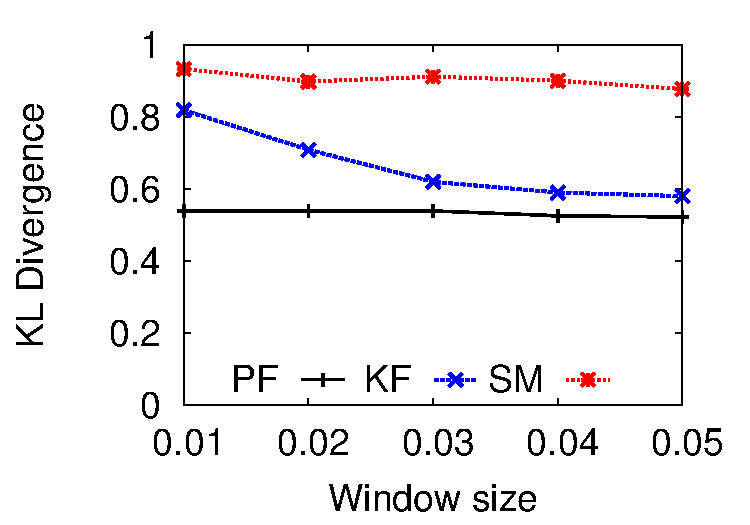
\includegraphics[width=.5\textwidth]{img/kl-w.pdf}
\caption{\label{fig:window-size}
Effects of query window size.}
\end{figure}

\section{Effects of \(k\)}
\label{sec:org0bd629d}

In this experiment we evaluate the accuracy of \(k\)NN query
results with respect to the value of \(k\).  We choose 100 random
indoor locations as \(k\)NN query points and issue queries on
these query points at 100 different time stamps.  As \(k\) goes
from 2 to 9, we can see in Figure \ref{fig:k} that the average hit rates
of Kalman filter-based and symbolic model-based methods grow
slowly.  As \(k\) increases, the number of objects returned by the
methods increase as well, resulting in a higher chance of hits.
On the contrary, the average hit rate of the particle filter-based
method is relatively stable with respect to the value of \(k\),
and the particle filter-based method always outperforms the other
two methods in terms of the average hit rate.

\begin{figure}[htbp]
\centering
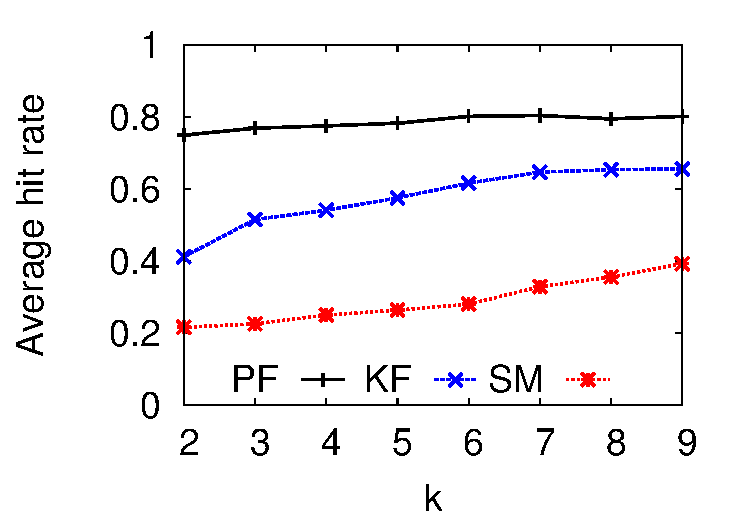
\includegraphics[width=.5\textwidth]{img/hit-k.pdf}
\caption{\label{fig:k}
Effects of \(k\)}
\end{figure}

\section{Effects of Number of Particles}
\label{sec:orgcfda28c}

From the mathematical analysis of particle filters in Section
\ref{sec:particle-filter}, we knew that if the number of particles is
too small, the accuracy of particle filters will degenerate due to
insufficient samples.  On the opposite, keeping a large number of
particles is not a good choice either since the computation cost
may become overwhelming, as the accuracy improvement is no longer
obvious when the number of particles is beyond a certain
threshold.  In this subsection, we conduct extensive experiments
to exploit the effects of the number of particles on query result
accuracy in order to determine an appropriate size of the particle
set for the application of indoor spatial queries.

\begin{figure}[h]
  \centering
  \begin{subfigure}{.5\linewidth}
    \centering
    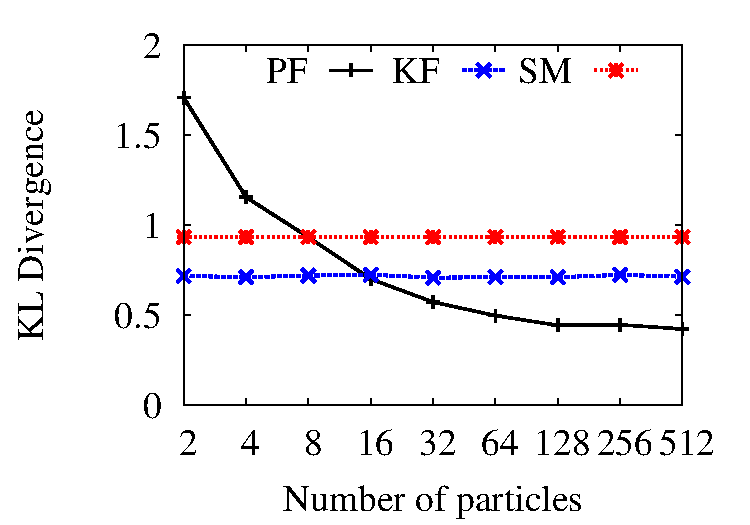
\includegraphics[width=\textwidth]{img/kl-p.pdf}
    \caption{KL divergence}
  \end{subfigure}%
  \begin{subfigure}{.5\linewidth}
    \centering
    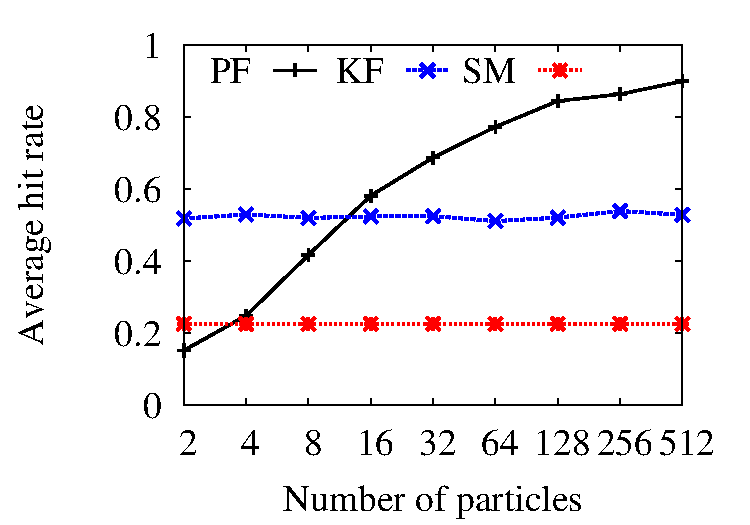
\includegraphics[width=\textwidth]{img/hit-p.pdf}
    \caption{\(k\)NN success ratio}
  \end{subfigure}
  \caption{The impact of the number of particles.}
  \label{fig:number-of-particles}
\end{figure}

As shown in Figure \ref{fig:number-of-particles}, we can see that
when the number of particles is very small, the particle
filter-based method has a larger KL divergence for range queries
and a smaller average hit rate for \(k\)NN queries than the other
two methods.  As the number of particles grows beyond 16, the
performance of the particle filter-based method exceeds the other
two.  However, the performance gain with more than 64 particles
slows down as we already have around 90\% accuracy.  Therefore, we
conclude that in our application, the appropriate size of the
particle set is around 60, which guarantees a good accuracy while
not costing too much in computation.

\section{Effects of Number of Moving Objects}
\label{sec:org75c6c55}


\begin{figure}[h]
  \centering
  \begin{subfigure}{.5\linewidth}
    \centering
    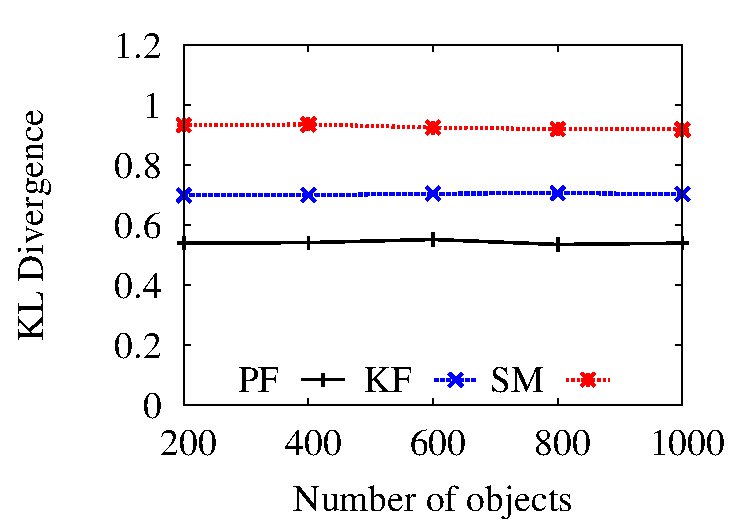
\includegraphics[width=\textwidth]{img/kl-n.pdf}
    \caption{KL divergence}
  \end{subfigure}%
  \begin{subfigure}{.5\linewidth}
    \centering
    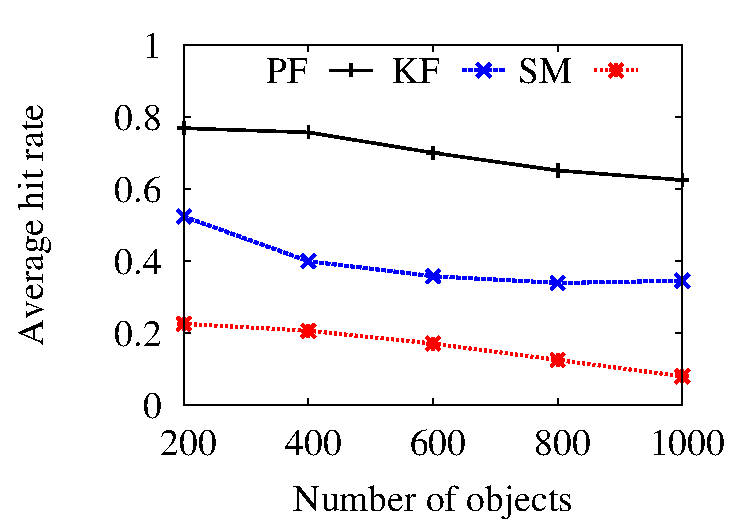
\includegraphics[width=\textwidth]{img/hit-n.pdf}
    \caption{\(k\)NN success ratio}
  \end{subfigure}
  \caption{The impact of the number of moving objects.}
  \vspace*{-5pt}
  \label{fig:number-of-objects}
\end{figure}

In this subsection, we evaluate the scalability of our proposed
algorithms by varying the number of moving objects from 200
to 1000.  All the result data are collected by averaging an
extensive number of queries over different query locations and
time stamps.  Figure \ref{fig:number-of-objects} shows that the KL
divergence of the three methods is relatively stable, while the
average hit rate of \(k\)NN queries decreases for all the methods.
The decrease of \(k\)NN hit rate is caused by increasing density
of objects.  A finer resolution algorithm is required to
accurately answer \(k\)NN queries.  In all, our solution
demonstrates good scalability in terms of accuracy when the number
of objects increases.

\section{Effects of Activation Range}
\label{sec:orge8c00a8}

\begin{figure}[h]
  \centering
  \begin{subfigure}{.5\linewidth}
    \centering
    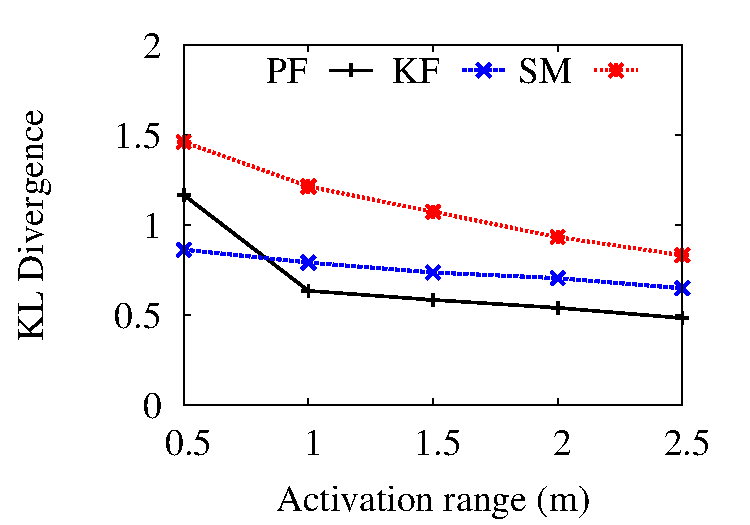
\includegraphics[width=\textwidth]{img/kl-r}
    \caption{KL divergence}
  \end{subfigure}%
  \begin{subfigure}{.5\linewidth}
    \centering
    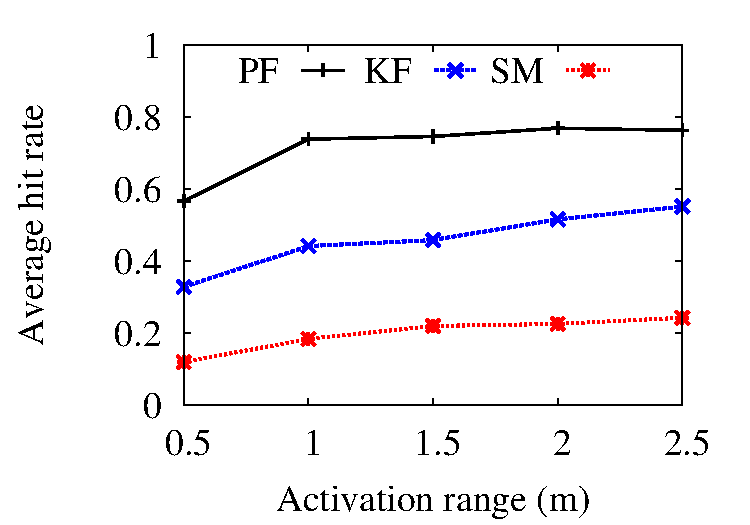
\includegraphics[width=\textwidth]{img/hit-r}
    \caption{\(k\)NN success ratio}
  \end{subfigure}
  \caption{The impact of activation range.}
  \label{fig:range}
\end{figure}

In this subsection, we evaluated the effects of reader's
activation range by varying the range from 50 cm to 250 cm.  The
results are reported in Figure \ref{fig:range}.  As the activation
range increases, the performance of all the three methods gets
better because uncertain regions not covered by any reader
essentially get reduced.  In addition, even when the activation
range is small (e.g., 100 cm), the particle filter-based method is
still able to achieve relatively high accuracy.  Therefore, the
particle filter-based method is more suitable than the other two
methods when the physical constraints limit readers' activation
ranges.

\section{Continuous Query Performance Evaluation}
\label{sec:orgb83268c}

The previous subsections show the performance of snapshot queries,
i.e., queries at a specific time stamp.  This subsection
demonstrates our algorithms' performance across a duration of
time.  The application scenarios are described as follows:

\begin{enumerate}
\item For continuous range query, a user registers a query window at
time \(t_0\), and unregisters at \(t_1\).  During the time
interval (between \(t_0\) and \(t_1\)), we keep updating the
user of the objects in the query window whenever a change is
detected.
\item For continuous \(k\)NN query, a user registers a query point
\(q\) on the walking graph (a query point which is not on the
walking graph can be projected to its closest edge of the
graph) at \(t_0\), and unregisters at \(t_1\).  During the time
interval, every time there is a change in the \(k\) nearest
neighbor query result set, we will update the user with the new
query result.

We develop two criteria to measure the performance
\begin{description}
\item[{Change Volume}] It is defined as the number of changes of
objects in the query range between two consecutive time
stamps, including departing and arriving objects. Suppose at
\(t_0\), the objects in the query range are \(\{a, b, c\}\);
at \(t_1\), the result set changes to \(\{a, b, d\}\), then
the number of changes equals to 2, because one of the
objects, \(c\), is departing and another object, \(d\), just
arrived.  The rationale behind this is that higher change
volume could potentially impair query result accuracy.
\item[{Query Duration}] It is the interval between \(t_0\) and
\(t_1\), where \(t_0\) denotes the time a user registers a
continuous query, and \(t_1\) denotes the time a user
unregisters the query.  The rationale for this criteria is
that the proposed algorithms can be evaluated as stable and
reliable if they can maintain a satisfactory accuracy for a
long duration.
\end{description}
\end{enumerate}


\begin{figure}[htbp]
\centering
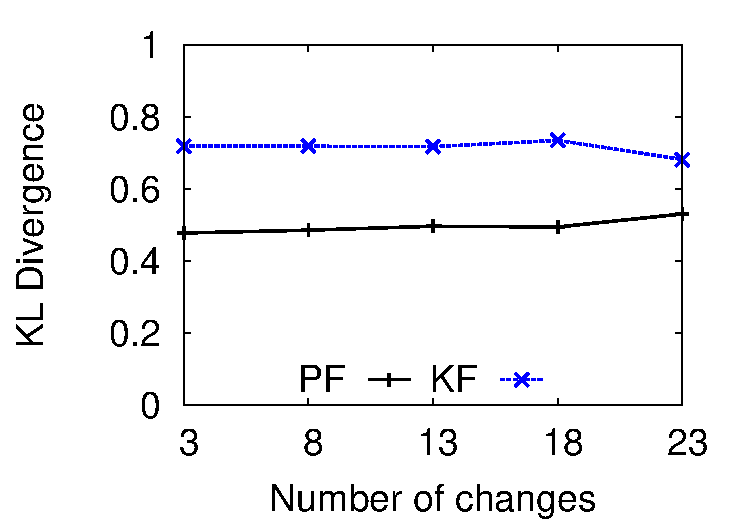
\includegraphics[width=.5\textwidth]{img/cont-kl-n.pdf}
\caption{\label{fig:cont-number-of-changes}
The impact of number of changes.}
\end{figure}

Figure \ref{fig:cont-number-of-changes} shows the performance of our
proposed algorithms with different number of changes.  It is clear
from the figure that our algorithms' accuracy is not heavily
influenced by the change volume, although there are some
fluctuations.  Furthermore, Figure \ref{fig:cont-duration} shows the
accuracy of our algorithms against the query duration.  Once the
system is stable, the accuracy of our algorithms is not affected
by the duration of query time.

\begin{figure}[h]
  \centering
  \begin{subfigure}{.5\linewidth}
    \centering
    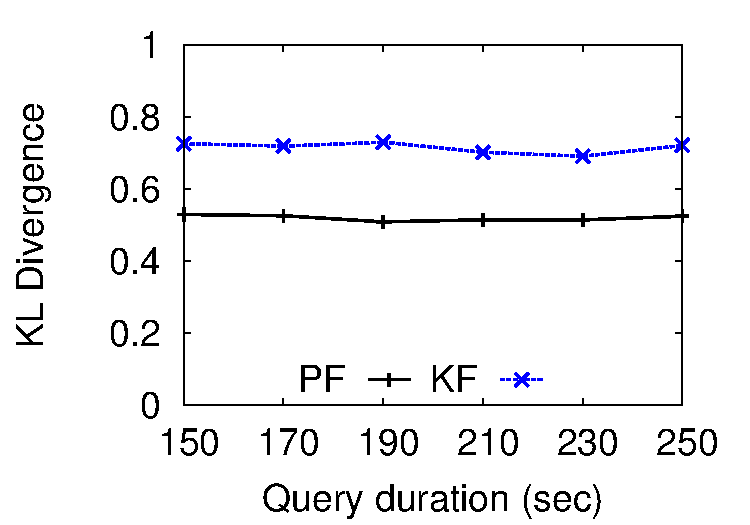
\includegraphics[width=\textwidth]{img/cont-kl-t.pdf}
    \caption{Continuous range query}
  \end{subfigure}%
  \begin{subfigure}{.5\linewidth}
    \centering
    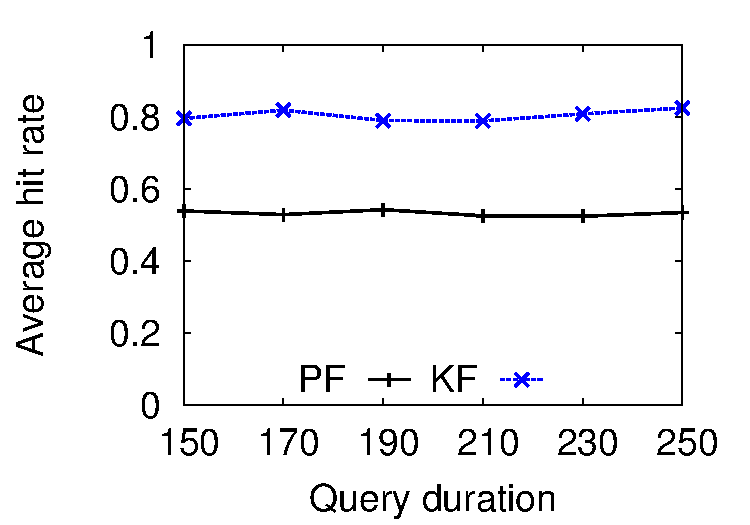
\includegraphics[width=\textwidth]{img/cont-hit-t.pdf}
    \caption{Continuous \(k\)NN query}
  \end{subfigure}
  \caption{The impact of query duration.}
  \label{fig:cont-duration}
\end{figure}

\part{Conclusion}
\label{sec:conclusion}
In this paper, we introduced a Bayesian filtering-based RFID data
cleansing method in order to support accurate indoor spatial queries
with noisy RFID data.  In addition we proposed the indoor walking
graph model and the anchor point indexing model to simplify the
Bayesian filtering process.  After the cleansing, indoor range query
and \(k\)NN query can be evaluated efficiently and effectively via
our algorithms.  Our extensive experiment with data generated by
real-world parameters demonstrates that our solution outperforms the
symbolic model-based method by large margin in query result
accuracy.

There are, however, a few limitations in our current solutions which
will be addressed in our future work.  For example, current solution
are evaluated on synthesized data, We plan to conduct further
analysis of our system with real data collected in the RFID lab.  In
addition, we intend to extend our framework to support more spatial
query types such as spatial skyline, spatial joins, closest-pairs,
etc.


\bibliographystyle{unsrt}
\bibliography{thesis}
\end{document}